% Options for packages loaded elsewhere
\PassOptionsToPackage{unicode}{hyperref}
\PassOptionsToPackage{hyphens}{url}
%
\documentclass[
]{article}
\usepackage{amsmath,amssymb}
\usepackage{lmodern}
\usepackage{iftex}
\ifPDFTeX
  \usepackage[T1]{fontenc}
  \usepackage[utf8]{inputenc}
  \usepackage{textcomp} % provide euro and other symbols
\else % if luatex or xetex
  \usepackage{unicode-math}
  \defaultfontfeatures{Scale=MatchLowercase}
  \defaultfontfeatures[\rmfamily]{Ligatures=TeX,Scale=1}
\fi
% Use upquote if available, for straight quotes in verbatim environments
\IfFileExists{upquote.sty}{\usepackage{upquote}}{}
\IfFileExists{microtype.sty}{% use microtype if available
  \usepackage[]{microtype}
  \UseMicrotypeSet[protrusion]{basicmath} % disable protrusion for tt fonts
}{}
\makeatletter
\@ifundefined{KOMAClassName}{% if non-KOMA class
  \IfFileExists{parskip.sty}{%
    \usepackage{parskip}
  }{% else
    \setlength{\parindent}{0pt}
    \setlength{\parskip}{6pt plus 2pt minus 1pt}}
}{% if KOMA class
  \KOMAoptions{parskip=half}}
\makeatother
\usepackage{xcolor}
\usepackage[margin=1in]{geometry}
\usepackage{color}
\usepackage{fancyvrb}
\newcommand{\VerbBar}{|}
\newcommand{\VERB}{\Verb[commandchars=\\\{\}]}
\DefineVerbatimEnvironment{Highlighting}{Verbatim}{commandchars=\\\{\}}
% Add ',fontsize=\small' for more characters per line
\usepackage{framed}
\definecolor{shadecolor}{RGB}{248,248,248}
\newenvironment{Shaded}{\begin{snugshade}}{\end{snugshade}}
\newcommand{\AlertTok}[1]{\textcolor[rgb]{0.94,0.16,0.16}{#1}}
\newcommand{\AnnotationTok}[1]{\textcolor[rgb]{0.56,0.35,0.01}{\textbf{\textit{#1}}}}
\newcommand{\AttributeTok}[1]{\textcolor[rgb]{0.77,0.63,0.00}{#1}}
\newcommand{\BaseNTok}[1]{\textcolor[rgb]{0.00,0.00,0.81}{#1}}
\newcommand{\BuiltInTok}[1]{#1}
\newcommand{\CharTok}[1]{\textcolor[rgb]{0.31,0.60,0.02}{#1}}
\newcommand{\CommentTok}[1]{\textcolor[rgb]{0.56,0.35,0.01}{\textit{#1}}}
\newcommand{\CommentVarTok}[1]{\textcolor[rgb]{0.56,0.35,0.01}{\textbf{\textit{#1}}}}
\newcommand{\ConstantTok}[1]{\textcolor[rgb]{0.00,0.00,0.00}{#1}}
\newcommand{\ControlFlowTok}[1]{\textcolor[rgb]{0.13,0.29,0.53}{\textbf{#1}}}
\newcommand{\DataTypeTok}[1]{\textcolor[rgb]{0.13,0.29,0.53}{#1}}
\newcommand{\DecValTok}[1]{\textcolor[rgb]{0.00,0.00,0.81}{#1}}
\newcommand{\DocumentationTok}[1]{\textcolor[rgb]{0.56,0.35,0.01}{\textbf{\textit{#1}}}}
\newcommand{\ErrorTok}[1]{\textcolor[rgb]{0.64,0.00,0.00}{\textbf{#1}}}
\newcommand{\ExtensionTok}[1]{#1}
\newcommand{\FloatTok}[1]{\textcolor[rgb]{0.00,0.00,0.81}{#1}}
\newcommand{\FunctionTok}[1]{\textcolor[rgb]{0.00,0.00,0.00}{#1}}
\newcommand{\ImportTok}[1]{#1}
\newcommand{\InformationTok}[1]{\textcolor[rgb]{0.56,0.35,0.01}{\textbf{\textit{#1}}}}
\newcommand{\KeywordTok}[1]{\textcolor[rgb]{0.13,0.29,0.53}{\textbf{#1}}}
\newcommand{\NormalTok}[1]{#1}
\newcommand{\OperatorTok}[1]{\textcolor[rgb]{0.81,0.36,0.00}{\textbf{#1}}}
\newcommand{\OtherTok}[1]{\textcolor[rgb]{0.56,0.35,0.01}{#1}}
\newcommand{\PreprocessorTok}[1]{\textcolor[rgb]{0.56,0.35,0.01}{\textit{#1}}}
\newcommand{\RegionMarkerTok}[1]{#1}
\newcommand{\SpecialCharTok}[1]{\textcolor[rgb]{0.00,0.00,0.00}{#1}}
\newcommand{\SpecialStringTok}[1]{\textcolor[rgb]{0.31,0.60,0.02}{#1}}
\newcommand{\StringTok}[1]{\textcolor[rgb]{0.31,0.60,0.02}{#1}}
\newcommand{\VariableTok}[1]{\textcolor[rgb]{0.00,0.00,0.00}{#1}}
\newcommand{\VerbatimStringTok}[1]{\textcolor[rgb]{0.31,0.60,0.02}{#1}}
\newcommand{\WarningTok}[1]{\textcolor[rgb]{0.56,0.35,0.01}{\textbf{\textit{#1}}}}
\usepackage{graphicx}
\makeatletter
\def\maxwidth{\ifdim\Gin@nat@width>\linewidth\linewidth\else\Gin@nat@width\fi}
\def\maxheight{\ifdim\Gin@nat@height>\textheight\textheight\else\Gin@nat@height\fi}
\makeatother
% Scale images if necessary, so that they will not overflow the page
% margins by default, and it is still possible to overwrite the defaults
% using explicit options in \includegraphics[width, height, ...]{}
\setkeys{Gin}{width=\maxwidth,height=\maxheight,keepaspectratio}
% Set default figure placement to htbp
\makeatletter
\def\fps@figure{htbp}
\makeatother
\setlength{\emergencystretch}{3em} % prevent overfull lines
\providecommand{\tightlist}{%
  \setlength{\itemsep}{0pt}\setlength{\parskip}{0pt}}
\setcounter{secnumdepth}{5}
\ifLuaTeX
  \usepackage{selnolig}  % disable illegal ligatures
\fi
\IfFileExists{bookmark.sty}{\usepackage{bookmark}}{\usepackage{hyperref}}
\IfFileExists{xurl.sty}{\usepackage{xurl}}{} % add URL line breaks if available
\urlstyle{same} % disable monospaced font for URLs
\hypersetup{
  pdftitle={HUDM6122 Homework\_05},
  pdfauthor={Chenguang Pan},
  hidelinks,
  pdfcreator={LaTeX via pandoc}}

\title{HUDM6122 Homework\_05}
\author{Chenguang Pan}
\date{2023-03-20}

\begin{document}
\maketitle

\hypertarget{github-address}{%
\subsection{Github Address}\label{github-address}}

All my latest homework can be found on Github:
\url{https://github.com/cgpan/hudm6122_homeworks} . Thanks for checking
if interested.

\hypertarget{ex-5.1}{%
\subsection{Ex 5.1}\label{ex-5.1}}

\emph{Show how the result rises from the assumptions of uncorrelated
factors, independence of the specific variates, and independence of
common factors and specific variances. What form does take if the
factors are allowed to be correlated?}

\textbf{MY SOLUTION:}\\
Based on the assumption of Exploratory Factor Analysis(EFA), a set of
observed variables \textbf{x} assumed to be linked to a set of latent
variables \textbf{f}. Therefore, we can have a regression model in
matrix form
\[\boldsymbol x=\boldsymbol\Lambda \boldsymbol f + \boldsymbol u\],
where \(\boldsymbol \Lambda\) is a \(q \times k\) matrix of factor
loadings (a.k.a., the coefficients of the regression model), and the
\emph{u} is the vector of unexplained error of each observed variables.

Let's take the variance of the formula above
\[V(\boldsymbol x) = V(\boldsymbol\Lambda \boldsymbol f + \boldsymbol u)\].
Based on the operation rule of variance, like
\[V(a+b)= V(a) + V(b) + 2Cov(ab)\], we combined the two formulas above,
then
\[V(\boldsymbol x) = V(\boldsymbol\Lambda \boldsymbol f + \boldsymbol u) = V(\boldsymbol\Lambda \boldsymbol f) + V(\boldsymbol u) + 2 Cov(\boldsymbol\Lambda \boldsymbol f \boldsymbol u)\].
Since the we assumed that the error terms are uncorrelated with the
factors, therefore the
\(Cov(\boldsymbol\Lambda \boldsymbol f \boldsymbol u)=0\). Then, we can
continue to drive the variance formula as
\[V(\boldsymbol x) = V(\boldsymbol\Lambda \boldsymbol f) + V(\boldsymbol u) = \boldsymbol\Lambda V(\boldsymbol f) \boldsymbol\Lambda^T + \Psi\].
In addition, we assumed that the factors are uncorrelated with each
other. The \(V(\boldsymbol f)\) is actually an identity matrix.
Therefore, the formula can be written as
\[V(\boldsymbol x) = \boldsymbol\Lambda V(\boldsymbol f) \boldsymbol\Lambda^T + \Psi = \boldsymbol\Lambda \boldsymbol\Lambda^T + \Psi\].
Finally, the formula can be written as
\[\boldsymbol \Sigma = \boldsymbol\Lambda \boldsymbol\Lambda^T + \Psi\].

If we allow the factors to be correlated with each other, then the
\(V(\boldsymbol f)\) is not an identity matrix. Let's use the greek
letter \(\Phi\) to represent the variance matrix of loadings \textbf{f}.
Thus, the formula should be
\[\boldsymbol \Sigma = \boldsymbol\Lambda \boldsymbol \Phi \boldsymbol\Lambda^T + \Psi\].

\hypertarget{ex-5.2}{%
\subsection{Ex 5.2}\label{ex-5.2}}

\emph{Show that the communalities in a factor analysis model are
unaffected by the transformation \ldots{}}

\textbf{MY SOLUTION:}\\
This question mentioned that we need to use the transformed factor
loadings \(\boldsymbol \Lambda ^* = \boldsymbol \Lambda \boldsymbol M\).
Let's assume that \(\boldsymbol M\) is an \(k \times k\) orthogonal
matrix. We can re-write the the basic regression equation linking the
observed and the factors as:
\[\boldsymbol x=(\boldsymbol\Lambda \boldsymbol M)( \boldsymbol M^T \boldsymbol f) + \boldsymbol u\].\\
Using the rule of variance, we can have
\[\boldsymbol \Sigma = (\boldsymbol\Lambda \boldsymbol M)(\boldsymbol\Lambda \boldsymbol M)^T + \Psi\].
Since the \(\boldsymbol M\) is a orthogonal matrix and
\(\boldsymbol M \boldsymbol M^T = \boldsymbol I\). Therefore, the
variance equation can be written as
\[\boldsymbol \Sigma = \boldsymbol\Lambda \boldsymbol\Lambda^T + \Psi\].
That is, the transformed factor loadings
\(\boldsymbol \Lambda ^* = \boldsymbol \Lambda \boldsymbol M\) will not
influence the communalities (i.e.,
\(\boldsymbol\Lambda \boldsymbol\Lambda^T\)) in the a factor analysis
model.

\hypertarget{ex-5.3}{%
\subsection{Ex 5.3}\label{ex-5.3}}

\emph{Give a formula for the proportion of variance explained by the jth
factor estimated by the principal factor approach.}

\textbf{MY SOLUTION:}\\
The proportion of variance explained by the jth factor represents the
proportion of the total variance in the observed variables that is
accounted for by that factor alone. Therefore, the formula could be
\[Proportion_j = \frac {\sum_{i=1}^{q} \lambda_{ij}^2}{\boldsymbol \Lambda \boldsymbol \Lambda ^T}\].

\hypertarget{ex-5.4}{%
\subsection{Ex 5.4}\label{ex-5.4}}

\emph{Apply the factor analysis model separately to the life
expectancies of men and women and compare the results.}

\textbf{MY SOLUTION:}\\
The textbook does not provide the original dataset. Based on the code in
the \texttt{MVA}, I create the dataset via a separated r file named
``HW05 Test''. This file created the \texttt{life.rdata} and
\texttt{life.csv} dataset in the same file folder.

\begin{Shaded}
\begin{Highlighting}[]
\SpecialCharTok{\textgreater{}} \FunctionTok{load}\NormalTok{(}\StringTok{"life.rdata"}\NormalTok{)}
\SpecialCharTok{\textgreater{}} \FunctionTok{head}\NormalTok{(life)}
\NormalTok{           m0 m25 m50 m75 w0 w25 w50 w75}
\NormalTok{Algeria    }\DecValTok{63}  \DecValTok{51}  \DecValTok{30}  \DecValTok{13} \DecValTok{67}  \DecValTok{54}  \DecValTok{34}  \DecValTok{15}
\NormalTok{Cameroon   }\DecValTok{34}  \DecValTok{29}  \DecValTok{13}   \DecValTok{5} \DecValTok{38}  \DecValTok{32}  \DecValTok{17}   \DecValTok{6}
\NormalTok{Madagascar }\DecValTok{38}  \DecValTok{30}  \DecValTok{17}   \DecValTok{7} \DecValTok{38}  \DecValTok{34}  \DecValTok{20}   \DecValTok{7}
\NormalTok{Mauritius  }\DecValTok{59}  \DecValTok{42}  \DecValTok{20}   \DecValTok{6} \DecValTok{64}  \DecValTok{46}  \DecValTok{25}   \DecValTok{8}
\NormalTok{Reunion    }\DecValTok{56}  \DecValTok{38}  \DecValTok{18}   \DecValTok{7} \DecValTok{62}  \DecValTok{46}  \DecValTok{25}  \DecValTok{10}
\NormalTok{Seychelles }\DecValTok{62}  \DecValTok{44}  \DecValTok{24}   \DecValTok{7} \DecValTok{69}  \DecValTok{50}  \DecValTok{28}  \DecValTok{14}
\SpecialCharTok{\textgreater{}} 
\ErrorTok{\textgreater{}} \CommentTok{\# subset the male and female dataset}
\ErrorTok{\textgreater{}}\NormalTok{ life\_male }\OtherTok{\textless{}{-}}\NormalTok{ life[,}\DecValTok{1}\SpecialCharTok{:}\DecValTok{4}\NormalTok{]}
\SpecialCharTok{\textgreater{}}\NormalTok{ life\_female }\OtherTok{\textless{}{-}}\NormalTok{ life[,}\DecValTok{5}\SpecialCharTok{:}\DecValTok{8}\NormalTok{]}
\SpecialCharTok{\textgreater{}} 
\ErrorTok{\textgreater{}} \CommentTok{\# test the number of factors needed for the male and female dataset separately}
\ErrorTok{\textgreater{}} \FunctionTok{sapply}\NormalTok{(}\DecValTok{1}\NormalTok{, }\ControlFlowTok{function}\NormalTok{(f)}
\SpecialCharTok{+}   \FunctionTok{factanal}\NormalTok{(life\_male, }\AttributeTok{factors=}\NormalTok{f, }\AttributeTok{method=}\StringTok{"mle"}\NormalTok{)}\SpecialCharTok{$}\NormalTok{PVAL)}
\NormalTok{   objective }
\FloatTok{0.0007284301} 
\SpecialCharTok{\textgreater{}} \FunctionTok{sapply}\NormalTok{(}\DecValTok{1}\NormalTok{, }\ControlFlowTok{function}\NormalTok{(f)}
\SpecialCharTok{+}   \FunctionTok{factanal}\NormalTok{(life\_female, }\AttributeTok{factors=}\NormalTok{f, }\AttributeTok{method=}\StringTok{"mle"}\NormalTok{)}\SpecialCharTok{$}\NormalTok{PVAL)}
\NormalTok{   objective }
\FloatTok{4.738464e{-}12} 
\end{Highlighting}
\end{Shaded}

When test the number of the factors from 1 to larger number, there is
always a warning that
\texttt{N\ factors\ are\ too\ many\ for\ N\ variables}. More details can
be found on Page 143 of the textbook or here
\url{https://stats.stackexchange.com/questions/593452/efa-n-factors-are-too-many-for-n-variables}

The results suggest that an one-factor solution might be adequate to
account for the observed covariances in the data.

Next, I run the one-factor solution for both male and female datasets.

\begin{Shaded}
\begin{Highlighting}[]
\SpecialCharTok{\textgreater{}} \FunctionTok{factanal}\NormalTok{(life\_male, }\AttributeTok{factors =} \DecValTok{1}\NormalTok{, }\AttributeTok{method=}\StringTok{"mle"}\NormalTok{)}

\NormalTok{Call}\SpecialCharTok{:}
\FunctionTok{factanal}\NormalTok{(}\AttributeTok{x =}\NormalTok{ life\_male, }\AttributeTok{factors =} \DecValTok{1}\NormalTok{, }\AttributeTok{method =} \StringTok{"mle"}\NormalTok{)}

\NormalTok{Uniquenesses}\SpecialCharTok{:}
\NormalTok{   m0   m25   m50   m75 }
\FloatTok{0.594} \FloatTok{0.552} \FloatTok{0.005} \FloatTok{0.434} 

\NormalTok{Loadings}\SpecialCharTok{:}
\NormalTok{    Factor1}
\NormalTok{m0  }\FloatTok{0.638}  
\NormalTok{m25 }\FloatTok{0.669}  
\NormalTok{m50 }\FloatTok{0.998}  
\NormalTok{m75 }\FloatTok{0.752}  

\NormalTok{               Factor1}
\NormalTok{SS loadings      }\FloatTok{2.415}
\NormalTok{Proportion Var   }\FloatTok{0.604}

\NormalTok{Test of the hypothesis that }\DecValTok{1}\NormalTok{ factor is sufficient.}
\NormalTok{The chi square statistic is }\FloatTok{14.45}\NormalTok{ on }\DecValTok{2}\NormalTok{ degrees of freedom.}
\NormalTok{The p}\SpecialCharTok{{-}}\NormalTok{value is }\FloatTok{0.000728} 
\SpecialCharTok{\textgreater{}} \FunctionTok{factanal}\NormalTok{(life\_female, }\AttributeTok{factors =} \DecValTok{1}\NormalTok{, }\AttributeTok{method=}\StringTok{"mle"}\NormalTok{)}

\NormalTok{Call}\SpecialCharTok{:}
\FunctionTok{factanal}\NormalTok{(}\AttributeTok{x =}\NormalTok{ life\_female, }\AttributeTok{factors =} \DecValTok{1}\NormalTok{, }\AttributeTok{method =} \StringTok{"mle"}\NormalTok{)}

\NormalTok{Uniquenesses}\SpecialCharTok{:}
\NormalTok{   w0   w25   w50   w75 }
\FloatTok{0.220} \FloatTok{0.005} \FloatTok{0.115} \FloatTok{0.526} 

\NormalTok{Loadings}\SpecialCharTok{:}
\NormalTok{    Factor1}
\NormalTok{w0  }\FloatTok{0.883}  
\NormalTok{w25 }\FloatTok{0.998}  
\NormalTok{w50 }\FloatTok{0.941}  
\NormalTok{w75 }\FloatTok{0.689}  

\NormalTok{               Factor1}
\NormalTok{SS loadings      }\FloatTok{3.134}
\NormalTok{Proportion Var   }\FloatTok{0.784}

\NormalTok{Test of the hypothesis that }\DecValTok{1}\NormalTok{ factor is sufficient.}
\NormalTok{The chi square statistic is }\FloatTok{52.15}\NormalTok{ on }\DecValTok{2}\NormalTok{ degrees of freedom.}
\NormalTok{The p}\SpecialCharTok{{-}}\NormalTok{value is }\FloatTok{4.74e{-}12} 
\end{Highlighting}
\end{Shaded}

\hypertarget{ex-5.6}{%
\subsection{Ex 5.6}\label{ex-5.6}}

\emph{The matrix below shows the correlations between ratings on nine
statements about pain made by 123 people suffering from extreme pain.
Each statement was scored on a scale from 1 to 6, ranging from agreement
to disagreement. The nine pain statements were as follows:}

\textbf{MY SOLUTION:}\\
First, to change the lower triangular matrix into the complete
correlation matrix.

\begin{Shaded}
\begin{Highlighting}[]
\SpecialCharTok{\textgreater{}} \FunctionTok{library}\NormalTok{(Matrix)}
\SpecialCharTok{\textgreater{}} \CommentTok{\# import the correlation matrix}
\ErrorTok{\textgreater{}}\NormalTok{ corr\_lower }\OtherTok{\textless{}{-}} \FunctionTok{matrix}\NormalTok{(}\FunctionTok{c}\NormalTok{(}\DecValTok{1}\NormalTok{, }\DecValTok{0}\NormalTok{, }\DecValTok{0}\NormalTok{, }\DecValTok{0}\NormalTok{, }\DecValTok{0}\NormalTok{, }\DecValTok{0}\NormalTok{, }\DecValTok{0}\NormalTok{, }\DecValTok{0}\NormalTok{, }\DecValTok{0}\NormalTok{,}
\SpecialCharTok{+}                       \SpecialCharTok{{-}}\FloatTok{0.04}\NormalTok{, }\DecValTok{1}\NormalTok{, }\DecValTok{0}\NormalTok{,}\DecValTok{0}\NormalTok{,}\DecValTok{0}\NormalTok{,}\DecValTok{0}\NormalTok{,}\DecValTok{0}\NormalTok{,}\DecValTok{0}\NormalTok{,}\DecValTok{0}\NormalTok{,}
\SpecialCharTok{+}                       \FloatTok{0.61}\NormalTok{, }\SpecialCharTok{{-}}\FloatTok{0.07}\NormalTok{, }\DecValTok{1}\NormalTok{,}\DecValTok{0}\NormalTok{,}\DecValTok{0}\NormalTok{,}\DecValTok{0}\NormalTok{,}\DecValTok{0}\NormalTok{,}\DecValTok{0}\NormalTok{,}\DecValTok{0}\NormalTok{,}
\SpecialCharTok{+}                       \FloatTok{0.45}\NormalTok{, }\SpecialCharTok{{-}}\FloatTok{0.12}\NormalTok{, }\FloatTok{0.59}\NormalTok{, }\DecValTok{1}\NormalTok{,}\DecValTok{0}\NormalTok{,}\DecValTok{0}\NormalTok{,}\DecValTok{0}\NormalTok{,}\DecValTok{0}\NormalTok{,}\DecValTok{0}\NormalTok{,}
\SpecialCharTok{+}                       \FloatTok{0.03}\NormalTok{, }\FloatTok{0.49}\NormalTok{, }\FloatTok{0.03}\NormalTok{, }\SpecialCharTok{{-}}\FloatTok{0.08}\NormalTok{, }\DecValTok{1}\NormalTok{,}\DecValTok{0}\NormalTok{,}\DecValTok{0}\NormalTok{,}\DecValTok{0}\NormalTok{,}\DecValTok{0}\NormalTok{,}
\SpecialCharTok{+}                       \SpecialCharTok{{-}}\FloatTok{0.29}\NormalTok{, }\FloatTok{0.43}\NormalTok{, }\SpecialCharTok{{-}}\FloatTok{0.13}\NormalTok{, }\SpecialCharTok{{-}}\FloatTok{0.21}\NormalTok{, }\FloatTok{0.47}\NormalTok{, }\DecValTok{1}\NormalTok{,}\DecValTok{0}\NormalTok{,}\DecValTok{0}\NormalTok{,}\DecValTok{0}\NormalTok{,}
\SpecialCharTok{+}                       \SpecialCharTok{{-}}\FloatTok{0.30}\NormalTok{, }\FloatTok{0.30}\NormalTok{, }\SpecialCharTok{{-}}\FloatTok{0.24}\NormalTok{, }\SpecialCharTok{{-}}\FloatTok{0.19}\NormalTok{, }\FloatTok{0.41}\NormalTok{, }\FloatTok{0.63}\NormalTok{,}\DecValTok{1}\NormalTok{,}\DecValTok{0}\NormalTok{,}\DecValTok{0}\NormalTok{, }
\SpecialCharTok{+}                       \FloatTok{0.45}\NormalTok{, }\SpecialCharTok{{-}}\FloatTok{0.31}\NormalTok{,}\FloatTok{0.59}\NormalTok{,}\FloatTok{0.63}\NormalTok{,}\SpecialCharTok{{-}}\FloatTok{0.14}\NormalTok{,}\SpecialCharTok{{-}}\FloatTok{0.13}\NormalTok{,}\SpecialCharTok{{-}}\FloatTok{0.26}\NormalTok{,}\DecValTok{1}\NormalTok{,}\DecValTok{0}\NormalTok{,}
\SpecialCharTok{+}                       \FloatTok{0.30}\NormalTok{,}\SpecialCharTok{{-}}\FloatTok{0.17}\NormalTok{,}\SpecialCharTok{{-}}\FloatTok{0.32}\NormalTok{,}\FloatTok{0.37}\NormalTok{,}\SpecialCharTok{{-}}\FloatTok{0.24}\NormalTok{,}\SpecialCharTok{{-}}\FloatTok{0.15}\NormalTok{,}\SpecialCharTok{{-}}\FloatTok{0.29}\NormalTok{,}\FloatTok{0.40}\NormalTok{,}\DecValTok{1}\NormalTok{),}\DecValTok{9}\NormalTok{,}\DecValTok{9}\NormalTok{, }\AttributeTok{byrow =}\NormalTok{ T)}
\SpecialCharTok{\textgreater{}} \CommentTok{\# generate a complete correlation matrix}
\ErrorTok{\textgreater{}}\NormalTok{ corr\_symmetric }\OtherTok{\textless{}{-}} \FunctionTok{forceSymmetric}\NormalTok{(corr\_lower, }\AttributeTok{uplo=}\StringTok{"L"}\NormalTok{)}
\end{Highlighting}
\end{Shaded}

The correlation matrix looks good. Next, I run the PCA first.

\begin{Shaded}
\begin{Highlighting}[]
\SpecialCharTok{\textgreater{}} \CommentTok{\# run the PCA first}
\ErrorTok{\textgreater{}} \CommentTok{\# use prcomp to calculate the principal components}
\ErrorTok{\textgreater{}}\NormalTok{ pca }\OtherTok{\textless{}{-}} \FunctionTok{prcomp}\NormalTok{(corr\_symmetric, }\AttributeTok{scale. =} \ConstantTok{FALSE}\NormalTok{)}
\SpecialCharTok{\textgreater{}} \CommentTok{\# get the PCA results}
\ErrorTok{\textgreater{}} \FunctionTok{summary}\NormalTok{(pca)}
\NormalTok{Importance of components}\SpecialCharTok{:}
\NormalTok{                          PC1    PC2     PC3     PC4    PC5     PC6     PC7}
\NormalTok{Standard deviation     }\FloatTok{1.1594} \FloatTok{0.5014} \FloatTok{0.31822} \FloatTok{0.18698} \FloatTok{0.1734} \FloatTok{0.15725} \FloatTok{0.09446}
\NormalTok{Proportion of Variance }\FloatTok{0.7466} \FloatTok{0.1396} \FloatTok{0.05624} \FloatTok{0.01942} \FloatTok{0.0167} \FloatTok{0.01373} \FloatTok{0.00496}
\NormalTok{Cumulative Proportion  }\FloatTok{0.7466} \FloatTok{0.8863} \FloatTok{0.94250} \FloatTok{0.96192} \FloatTok{0.9786} \FloatTok{0.99235} \FloatTok{0.99730}
\NormalTok{                           PC8       PC9}
\NormalTok{Standard deviation     }\FloatTok{0.06968} \FloatTok{3.631e{-}17}
\NormalTok{Proportion of Variance }\FloatTok{0.00270} \FloatTok{0.000e+00}
\NormalTok{Cumulative Proportion  }\FloatTok{1.00000} \FloatTok{1.000e+00}
\SpecialCharTok{\textgreater{}} \CommentTok{\# draw the scree plot }
\ErrorTok{\textgreater{}} \FunctionTok{plot}\NormalTok{(pca, }\AttributeTok{type =} \StringTok{"l"}\NormalTok{, }
\SpecialCharTok{+}      \AttributeTok{main =} \StringTok{"Scree Plot"}\NormalTok{)}
\end{Highlighting}
\end{Shaded}

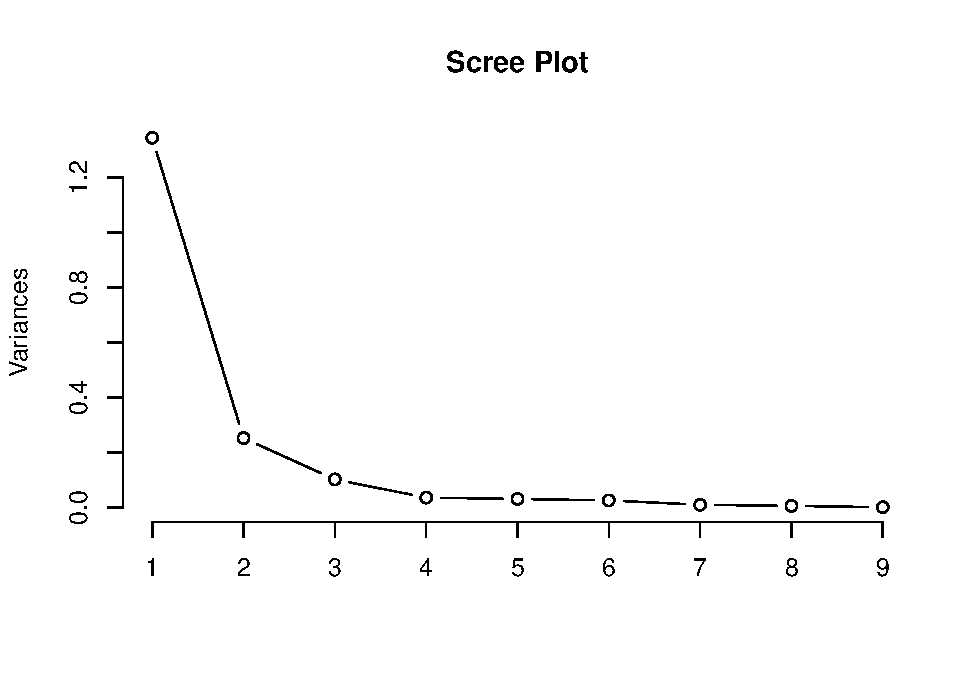
\includegraphics{HUDM6122-Homework_05-Chenguang-Pan_files/figure-latex/unnamed-chunk-4-1.pdf}

\end{document}
